\lhead{\textit{CAP\'ITULO \thechapter. Resultados}}
\chead{}
\rhead{\thepage}


\chapter{Resultados}
\section*{Introducci\'on}
\addcontentsline{toc}{section}{Introducci\'on}

En éste capítulo se describe los resultados obtenidos en modelado y simulación del centro de datos en CloudSim. 
Se ilustran por medio de gráficas lineales el tiempo de ejecución de los algoritmos de calendarización. Se representa en gráficas de barras el promedio del costo de procesamiento y tiempo de ejecución y una interpretación de la desviación estándar obtenida. La experimentación fue desarrollada en una computadora con un procesador \textit{Intel Core i5}, teniendo la siguiente configuración: \textit{2.5 GHz, 3 MB de cach\'e, 4 GB de RAM, Linux Ubuntu 14.04 LTS, 64 bits como sistema operativo y JDK 8.6}.






\vspace{20em} 

\section{Tiempo de ejecuci\'on y costo de procesamiento}


Para evaluar los algoritmos de calendarizaci\'on seleccionados se ha implementado un entorno de c\'omputo en la nube que consiste en un \textit{datacenter}, un \textit{broker}, m\'aquinas virtuales y \textit{host}.  Con el objetivo de evaluar el tiempo de ejecuci\'on y el costo de procesamiento en el \textit{datacenter} tras ejecutar cierto n\'umero de tareas \textit{(cloudlets)}.

Para la configuraci\'on del centro de datos en \textit{CloudSim} se utilizaron diez \textit{host}, cinco m\'aquinas virtuales por \textit{host} y las tareas fueron establecidas en un intervalo de 100 hasta 500 (Cuadro \ref{table:datacenter}).
Como se puede apreciar en el (Cuadro \ref{tab:host}), cada \textit{host} tuvo 2048 Mb de memoria RAM, dos n\'ucleos de procesamiento que tienen un almacenamiento de 800 GB \'o 1 TB, estas fueron elegidas de manera aleatoria y finalmente el ancho de banda fue de 1 GB/s.

\setcounter{table}{0}
\renewcommand\thetable{\arabic{table}}
\begin{table}[h!]
	\centering
	\begin{tabular}{@{}cc@{}}
		\toprule
		\multicolumn{2}{c}{{\bf Datacenter}} \\ \midrule
		Host              & 10               \\
		VM                & 5                \\
		Cloudlet          & 100-500          \\ \bottomrule
		
	\end{tabular}
	\caption{Configuraci\'on \textit{Datacenter}, Fuente: Elaboraci\'on propia.}
	\label{table:datacenter}
\end{table}
 
\setcounter{table}{1}
\renewcommand\thetable{\arabic{table}}
\begin{table}[h!]
	\centering
	\begin{tabular}{@{}cc@{}}
		\toprule
		\multicolumn{2}{c}{{\bf Host}} \\ \midrule
		RAM           & 2048 MB        \\
		CPU           & 2              \\
		Storage       & 800GB-1TB      \\ \midrule
		BW            & 1 GB/s        
	\end{tabular}
	\caption{Configuraci\'on de \textit{Host}, Fuente: Elaboraci\'on propia.}
	\label{tab:host}
\end{table}

\newpage

\setcounter{table}{2}
\renewcommand\thetable{\arabic{table}}
\begin{table}[h!]
	\centering
	\begin{tabular}{@{}cc@{}}
		\toprule
		\multicolumn{2}{c}{{\bf VirtualMachine}} \\ \midrule
		RAM               & 512 MB| 1GB          \\
		MIPS              & 250 | 500            \\
		Storage           & 10 GB                \\ \midrule
		BW                & 1 GB/s              
	\end{tabular}
	\caption{\textit{Virtual Machine}, Fuente: Elaboraci\'on propia.}
	\label{tab:machine}
\end{table}


\setcounter{table}{3}
\renewcommand\thetable{\arabic{table}}
\begin{table}[h!]
	\centering
	\begin{tabular}{@{}cc@{}}
		\toprule
		\multicolumn{2}{c}{{\bf Cloudlet}} \\ \midrule
		length           & 1kb-10kb        \\
		MIPSlength       & 300b-1.8kb      \\
		length           & 300b-1.8kb      \\ \midrule
		length           & 1000 kb/s      
	\end{tabular}
	\caption{Configuraci\'on \textit{Cloudlet}, Fuente: Elaboraci\'on propia.}
	\label{tab:cloudlet}
\end{table}


En el Cuadro (\ref{tab:machine}) se muestran los par\'ametros que se consider\'o para las m\'aquinas virtuales, donde cada \textit{VM} tendr\'a 10 GB de almacenamiento, 512 MB  o 1 GB seleccionado de manera aleatoria, adem\'as para la caracter\'istica del procesador se tiene  la propiedad \textit{MIPS} \textit{(million instructions per second)} con 250 \'o 500 y un ancho de banda de 1000 kb/s.

Para la configuraci\'on de las tareas, se tom\'o el tamaño con un intervalo de 1 kb a 10 kb,  el par\'ametro \textit{fileSize}, que representa el tamaño del archivo de entrada, va de 300 b a 1.8 kb as\'i como el archivo de salida, como par\'ametro final se tiene los \textit{MIPS} que ir\'an de 1 a 3 (Cuadro \ref{tab:cloudlet}).



\newpage

\setcounter{figure}{17}
\renewcommand\thefigure{\arabic{figure}}
\begin{figure}[h!] 
	\centering
	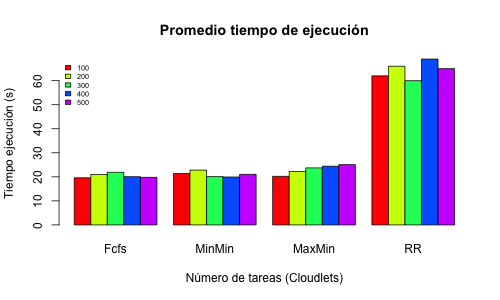
\includegraphics[scale=0.5]{media/tiempoejecucion}
	\caption{Promedio tiempo de ejecuci\'on con tareas 100-500, Fuente: Elaboraci\'on propia.}
	\label{fig:tiempo}
\end{figure}



En la figura (\ref{fig:tiempo}), se puede observar el promedio del tiempo de ejecuci\'on en \emph{ms} para diferentes cantidades de tareas (de 100 a 500). A primera vista con el algoritmo \textit{FCFS} y \textit{Min-Min} se mantiene un tiempo de ejecuci\'on sin muchos cambios a pesar del aumento en la carga de tareas, a diferencia del algoritmo \textit{Max-Min} que aument\'o el tiempo de ejecuci\'on a medida que se increment\'o el n\'umero de tareas.

\label{etiqueta}
\newpage

\setcounter{figure}{18}
\renewcommand\thefigure{\arabic{figure}}
\begin{figure}[h!] 
	\centering
	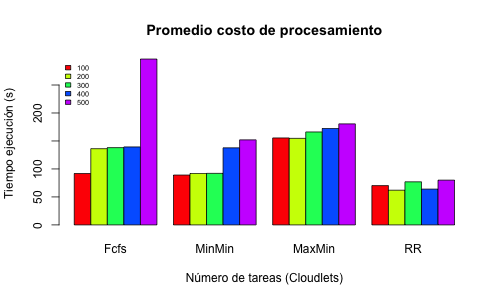
\includegraphics[scale=0.5]{media/costoproce}
	\caption{Promedio costo de procesamiento con tareas 100-500, Fuente: Elaboraci\'on propia.}
	\label{fig:costo}
\end{figure}


El costo de procesamiento, de acuerdo a cada algoritmo, se puede observar en la figura (\ref{fig:costo}), en donde el algoritmo \textit{FCFS} tiene un incremento dr\'astico al realizar la prueba con 500 tareas. El algoritmo \textit{Max-Min} se conserv\'o sin muchos cambios apesar de la cantidad de tareas, mientras que \textit{Min-Min} tiene un menor costo de procesamiento cuando las tareas son inferiores a 300.
\label{etiqueta2}
\newpage

\setcounter{figure}{19}
\renewcommand\thefigure{\arabic{figure}}
\begin{figure}[h!] 
	\centering
	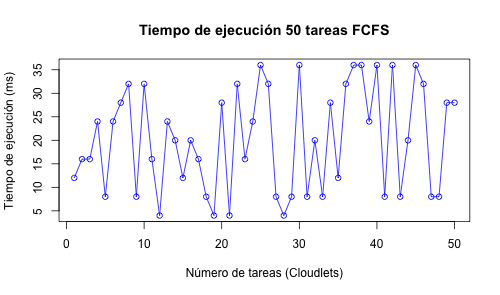
\includegraphics[scale=0.6]{media/fcfs}
	\caption{Tiempo ejecuci\'on 50 muestras \textit{FCFS}, Fuente: Elaboraci\'on propia.}
	\label{fig:ejecucion}
\end{figure}


Para mostrar el comportamiento del tiempo de ejecuci\'on por cada algoritmo, se tomaron 50 muestras de una simulaci\'on de 500 tareas. En la figura (\ref{fig:ejecucion}), se puede apreciar que el algoritmo \textit{FCFS} tiene un comportamiento inestable ya que algunas tareas pueden tener menor complejidad o tamaño, lo que implica una respuesta r\'apida.

\newpage

\setcounter{figure}{20}
\renewcommand\thefigure{\arabic{figure}}
\begin{figure}[h!] 
	\centering
	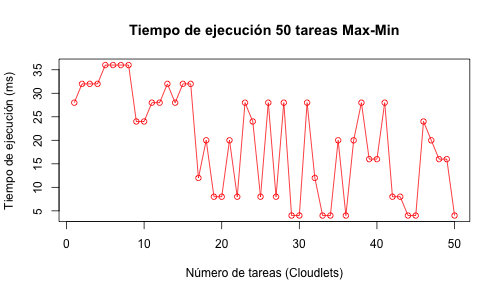
\includegraphics[scale=0.6]{media/maxmin}
	\caption{Tiempo ejecuci\'on 50 muestras \textit{Max-Min}, Fuente: Elaboraci\'on propia.}
	\label{fig:maxmin}
\end{figure}


 En la figura (\ref{fig:maxmin}) se tiene la misma simulaci\'on pero con el algoritmo \textit{Max-Min}, de acuerdo a las caracter\'isticas de este calendarizador, en las primeras tareas se toma un mayor tiempo en responder y va disminuyendo de manera gradual, sin embargo a\'un es inestable en las \'ultimas muestras ya que no se contempla el grado de complejidad, es decir el par\'ametro \textit{MIPS} de los \textit{cloudlets}.



\newpage
\setcounter{figure}{21}
\renewcommand\thefigure{\arabic{figure}}
\begin{figure}[h!] 
	\centering
	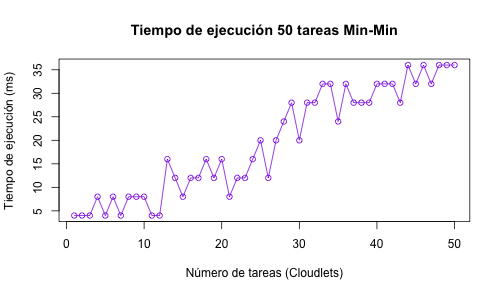
\includegraphics[scale=0.6]{media/minmin}
	\caption{Tiempo ejecuci\'on 50 muestras \textit{Min-Min}, Fuente: Elaboraci\'on propia.}
	\label{fig:minmin}
\end{figure}

En la parte de arriba se puede apreciar el algoritmo \textit{Min-Min} en el que el tiempo de ejecuci\'on fue aumentando conforme se resolv\'ian las tareas (figura \ref{fig:minmin}). Por último, en la figura (\ref{fig:roundrobin}) podemos visualizar la gráfica correspondiente al algoritmo \textit{Round Robin}.

\setcounter{figure}{22}
\renewcommand\thefigure{\arabic{figure}}
\begin{figure}[h!] 
	\centering
	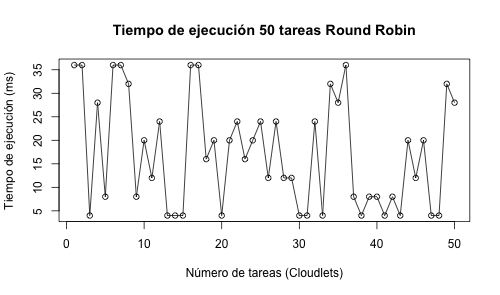
\includegraphics[scale=0.6]{media/roundrobin}
	\caption{Tiempo ejecuci\'on 50 muestras \textit{Round Robin}, Fuente: Elaboraci\'on propia.}
	\label{fig:roundrobin}
\end{figure}

\newpage



\setcounter{figure}{23}
\renewcommand\thefigure{\arabic{figure}}
\begin{figure}[h!] 
	\centering
	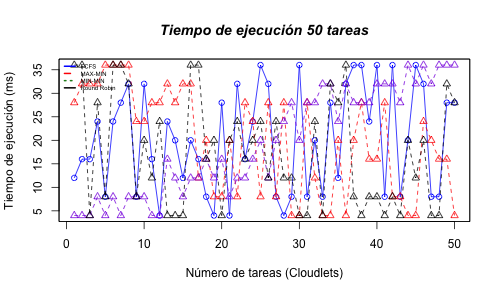
\includegraphics[scale=0.7]{media/figure}
	\caption{Tiempo ejecuci\'on 50 muestras de todos los algoritmos, Fuente: Elaboraci\'on propia.}
	\label{fig:figure}
\end{figure}

La figura (\ref{fig:figure}) muestra una comparativa de los cuatro algoritmos mostrados anteriormente. Durante la evaluación de los algoritmos se tomaron en cuenta dos datos estadísticos: la desviación estandar y el promedio que fue descrito en las páginas \pageref{etiqueta} y \pageref{etiqueta2}.


\setcounter{table}{4}
\renewcommand\thetable{\arabic{table}}
\begin{table}[h!]
	\centering
	\begin{tabular}{@{}cc@{}}
		\toprule
		{\bf Algoritmo} & \multicolumn{1}{l}{{\bf Desviaci\'on est\'andar}} \\ \midrule
		FCFS & 11.00619 \\
		MAX-MIN & 8.91444 \\
		MIN-MIN & 11.25613 \\ 
		ROUND ROBIN & 11.66722 \\ \bottomrule
		
	\end{tabular}
	\caption{Desviaci\'on est\'andar del tiempo de ejecuci\'on, Fuente: Elaboraci\'on propia.}
	\label{tiempotabla}
\end{table}

Observando la desviaci\'on est\'andar de \'estas muestras anteriores, los algoritmo \textit{Min-Min}, \textit{Round Robin} y \textit{FCFS} tuvieron m\'as variaciones en las muestras con respecto a la media, mientras que el \textit{Max-Min} tuvo las variaciones por debajo de las dos anteriores (Cuadro \ref{tiempotabla}).